\documentclass[pdflatex,sn-mathphys-num]{sn-jnl}% Springer Nature LaTeX template

\usepackage{amsmath,amssymb}
\usepackage{graphicx}
\usepackage{adjustbox}
\usepackage{booktabs}
% Typographic improvements and better line breaking
\usepackage[protrusion=true,expansion=true]{microtype}
\usepackage{xurl} % allow line breaks in long URLs/DOIs
\Urlmuskip=0mu plus 1mu
% Diagram
\usepackage{tikz}
\usetikzlibrary{arrows.meta,positioning,shapes.geometric}
\raggedbottom
% Mitigate overfull/underfull boxes in tight paragraphs
\setlength{\emergencystretch}{3em}

% Avoid hyperref bookmark warnings from \paragraph headings
\AtBeginDocument{\hypersetup{bookmarksdepth=3}}

\begin{document}

\title[Three-Stage Bearing Health Classification]{Three-Stage Bearing Health Classification Using Vibration Short-Time Fourier Transform and Temperature Trends in a Run-to-Failure Setting}

\author[1]{\fnm{Long} \sur{Truong}}\email{longt5@fpt.edu.vn}
\equalcont{These authors contributed equally to this work.}

\author*[2]{\fnm{Phu~Le} \sur{Nguyen}}\email{lpnguyen@ntt.edu.vn}
\equalcont{These authors contributed equally to this work.}

\affil[1]{\orgname{FPT University}, \orgaddress{\city{Ho Chi Minh City}, \country{Vietnam}}}
\affil[2]{\orgname{Faculty of Engineering and Technology, Nguyen Tat Thanh University}, \orgaddress{\city{Ho Chi Minh City}, \country{Vietnam}}}

\abstract{A lightweight multi-modal pipeline is presented for three-stage bearing health classification in run-to-failure settings. Vibration is converted to STFT spectrograms for a compact 2D CNN, and a minimal 6-D temperature trend/statistics descriptor is fused at a late head. Two design choices make the method practical and robust: per-frequency (across-time) normalization that stabilizes spectrogram brightness across windows, and file-wise mean-logit aggregation for stable decisions. A leakage-aware, time-to-failure\,\mbox{(TTF)}-aligned protocol and a two-phase training scheme (stratified pre-training then temporal fine-tuning) ground evaluation in deployment reality and reduce temporal leakage. The approach is simple (few parameters, AMP-friendly), efficient, and improves late-life discrimination compared with vibration-only baselines on a public run-to-failure dataset, providing actionable early warning while remaining easy to deploy.}

\keywords{bearing health monitoring, run-to-failure, degradation stage classification, STFT spectrogram, vibration--temperature fusion, temporal split, condition-based maintenance}

\maketitle
\section{Introduction}
\label{sec:intro}

Rotating machinery is a core asset in modern industry, and rolling-element bearings are among the most failure-prone components due to continuous mechanical stress, friction, and thermal loading. Unexpected bearing failures can cause unplanned downtime, safety risks, and substantial maintenance costs. Consequently, \emph{condition-based maintenance} (CBM) and \emph{prognostics and health management} (PHM) aim to continuously monitor bearing health and trigger maintenance actions before critical breakdowns.

Vibration-based diagnosis has been widely explored, where deep learning models---especially convolutional neural networks (CNNs)---learn discriminative patterns from raw waveforms or time--frequency representations such as spectrograms. However, practical CBM deployment often needs more than binary ``healthy vs.\ fault'' decisions. In run-to-failure monitoring, an intermediate \emph{degrading} stage is crucial for early warning, but it is also the hardest to recognize due to subtle signal changes, class imbalance, and evolving operating conditions \cite{jung2024dib_rtf}.

A second challenge is \emph{evaluation realism}. Many bearing diagnostic studies rely on random or window-level splits that inadvertently leak temporally adjacent samples across train/test, yielding overly optimistic performance \cite{kaufman2012leakage,bergmeir2012timeseriescv}. In real deployments, models must generalize from earlier-life behavior to later-life degradation patterns that were not observed during training. Therefore, leakage-aware temporal protocols aligned with the time-to-failure (TTF) axis are necessary to estimate true field performance.

Finally, multi-sensor information can improve stage recognition. Temperature is often correlated with friction and abnormal thermal behavior, providing complementary evidence to vibration signals, especially near degradation onset. Yet effectively fusing temperature with vibration while keeping the model lightweight remains non-trivial \cite{baltrusaitis2019multimodal}.

Three-stage bearing health classification (Healthy, Degrading, Fault) under a run-to-failure setting is addressed using vibration STFT representations and temperature trend descriptors \cite{jung2024dib_rtf,jung2024mendeley_rtf}. The key idea is to couple (i) time--frequency CNN features from vibration with (ii) compact temperature trend/statistical descriptors via a late-fusion classifier, and (iii) validate performance using leakage-aware temporal splits aligned with TTF.
To bridge development and deployment, a two-phase workflow is followed: first, a baseline model is trained under a file-wise stratified split, and then leakage-aware temporal fine-tuning aligned with the TTF axis is performed (train [0,60]\%, val [60,70]\%, test [70,100.1]\%). This design explicitly tests generalization from earlier-life behavior to later-life degradation while reducing the optimistic bias caused by temporally overlapped windows.
\textbf{Contributions.} This paper makes the following contributions, focusing on what is new and practically useful:
\begin{itemize}
    \item A compute-efficient multi-modal pipeline is proposed that fuses STFT-based two-axis vibration features with a minimal 6-D temperature trend/statistical descriptor via a late-fusion head, together with per-frequency (across-time) normalization to stabilize spectrogram brightness.
    \item A leakage-aware, TTF-aligned evaluation recipe with present-class scoring and file-wise mean-logit aggregation is employed to reflect deployment and avoid window-overlap leakage; the protocol makes performance interpretation robust when some classes are absent late in life.
    \item Targeted ablations (vibration-only vs. multi-modal, stratified initialization vs. scratch, temporal slice selection) are provided to explain when temperature adds value and how initialization affects temporal generalization.
    \item Empirically, strong performance is achieved: Macro-F1 $\approx$ 0.7762 on a 3-class stratified split; under leakage-aware late-life temporal testing with mean-logit aggregation, Early (70--90\%) Accuracy $=1.0000$ (Degrading only) and Late (90--100\%) Fault F1 $\approx$ 0.556, with clear gains over a vibration-only baseline in late-life Fault recognition.
\end{itemize}

\section{Related Works}
\label{sec:related_work}

Time--frequency CNNs are widely used for bearing diagnostics: vibration windows are mapped to spectrogram-like images and processed by compact 2D CNNs, yielding strong baselines in controlled settings \cite{zhao2019deep,lei2020roadmap,ince2016tie,wen2018neurocomputing}. In run-to-failure monitoring, however, recognizing an intermediate \emph{Degrading} stage is harder than binary fault detection due to subtle, evolving signatures and class imbalance. A well-known pitfall is optimistic bias from random/window-level splits with overlapped windows; near-duplicate content can leak across train/test. Leakage-aware temporal protocols aligned with the time-to-failure axis are therefore advocated to better match deployment, where future (later-life) data are unseen during training \cite{kaufman2012leakage,bergmeir2012timeseriescv}.

Multi-sensor fusion offers complementary evidence: temperature correlates with friction/thermal load and can improve robustness around degradation onset. Prior fusion studies support combining modalities for stronger diagnostics \cite{baltrusaitis2019multimodal,huo2022tim_multisensor,gao2024inffus_multisource,xiao2025inffus_multilevel}. Building on these ideas, we adopt two-axis STFT spectrograms with per-frequency normalization, fuse a minimal 6-D temperature trend/statistics descriptor via a late head, and evaluate with a leakage-aware temporal split on a public run-to-failure dataset \cite{jung2024dib_rtf,jung2024mendeley_rtf}. Our codebase adapts an open-source CNN implementation \cite{mdzalfirdausi_paderborn_repo} and tailors it to run-to-failure windowing, temperature fusion, and file-wise aggregation.

\section{Methodology}
\label{sec:method}

\subsection{Overview}
A lightweight multi-modal pipeline is proposed for bearing health stage recognition. For each 1.0-s window, two-axis vibration is transformed into a 2-channel log-spectrogram image and two-channel temperature is summarized into a compact 6-D descriptor. A small ResNet-style CNN encodes vibration patterns, a linear layer embeds temperature features, and a late-fusion classifier predicts the health stage. To bridge development and deployment, a two-phase workflow is adopted: stratified training followed by leakage-aware temporal fine-tuning along the TTF axis. Implementation-wise, code components are adapted from an open-source repository~\cite{mdzalfirdausi_paderborn_repo} and customized for TTF-aligned temporal splitting, per-window/per-frequency spectrogram normalization, temperature-fusion at the head, and file-wise mean-logit aggregation.

\subsection{Block Diagram}
Figure~\ref{fig:block} illustrates the end-to-end data flow from raw inputs to file-wise decisions and where fusion occurs.

\begin{figure}[t]
  \centering
  \begin{adjustbox}{max width=\linewidth}
  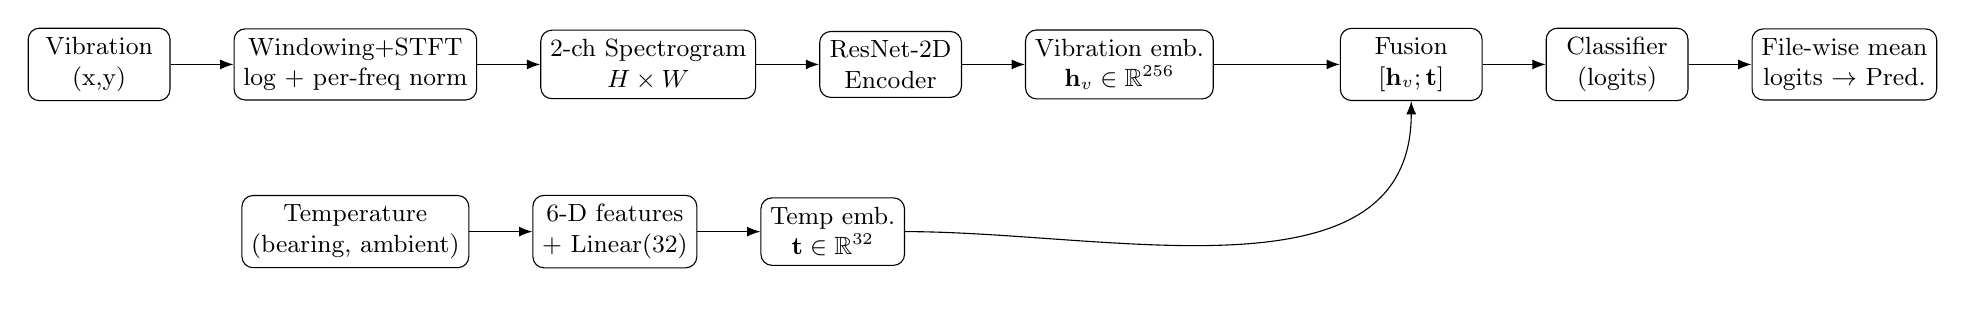
\begin{tikzpicture}[
    node distance=8mm and 8mm,
    box/.style={draw, rounded corners, align=center, minimum height=7mm, minimum width=18mm, font=\small},
    arr/.style={-Latex}
  ]
    % Top chain (compact)
    \node[box] (vib) {Vibration\\(x,y)};
    \node[box, right=of vib] (wstft) {Windowing+STFT\\log + per-freq norm};
    \node[box, right=of wstft] (spec) {2-ch Spectrogram\\$H\times W$};
    \node[box, right=of spec] (cnn) {ResNet-2D\\Encoder};
    \node[box, right=of cnn] (vz) {Vibration emb.\\$\mathbf{h}_v\in\mathbb{R}^{256}$};

    % Temp branch (compact)
    \node[box, below=12mm of wstft, xshift=0mm] (temp) {Temperature\\(bearing, ambient)};
    \node[box, right=of temp] (tfeat) {6-D features\\+ Linear(32)};
    \node[box, right=of tfeat] (tz) {Temp emb.\\$\mathbf{t}\in\mathbb{R}^{32}$};

    % Fusion + classifier + aggregation
    \node[box, right=16mm of vz] (fuse) {Fusion\\$[\mathbf{h}_v;\mathbf{t}]$};
    \node[box, right=of fuse] (cls) {Classifier\\(logits)};
    \node[box, right=of cls] (agg) {File-wise mean\\logits $\to$ Pred.};

    % Arrows top chain
    \draw[arr] (vib) -- (wstft);
    \draw[arr] (wstft) -- (spec);
    \draw[arr] (spec) -- (cnn);
    \draw[arr] (cnn) -- (vz);

    % Temp arrows
    \draw[arr] (temp) -- (tfeat);
    \draw[arr] (tfeat) -- (tz);

    % Fusion arrows
    \draw[arr] (vz) -- (fuse);
    % Route temp embedding to fusion from below to avoid crossing blocks
    \draw[arr] (tz.east) to[out=0,in=270] (fuse.south);
    \draw[arr] (fuse) -- (cls);
    \draw[arr] (cls) -- (agg);
  \end{tikzpicture}
  \end{adjustbox}
  \caption{Block diagram of the proposed multi-modal pipeline with late fusion and file-wise mean-logit aggregation.}
  \label{fig:block}
\end{figure}

\subsection{Synchronous windowing for vibration and temperature}
Vibration (2 axes) and temperature (2 channels) are sampled synchronously and sliced by identical 1.0-s windows with 50\% overlap, avoiding extra timestamp alignment. (If rates differ in deployment, a simple resampling/alignment step is required.)

\subsection{Preprocessing and spectrograms}
Each window is sanitized (NaN/Inf \,$\to$\,0) and z-scored per channel. STFT log-magnitude spectrograms are computed with $n\_{fft}=2048$, $hop\_length=512$ (Hann), then resized to $160\times160$.

\subsection{Per-frequency normalization and stacking}
To stabilize spectrogram "brightness" across frames, we apply per-frequency (across-time) normalization, then stack the two vibration axes as channels to form a $(2\times H\times W)$ input.

\subsection{Temperature descriptor (6-D) per window}
For temperature, we compute a compact 6-D descriptor (mean, std, slope for each channel) per window; non-finite values default to zero.

\vspace{2pt}

\subsection{Vibration encoder: lightweight ResNet-18 variant}
Spectrogram inputs are encoded with a compact ResNet-18-style \cite{he2016resnet} 2D CNN configured for two input channels. The stem uses a $7\times7$ convolution with stride 2 and 32 channels, followed by batch normalization, ReLU, and max pooling. Four stages of BasicBlocks follow with channel progression:
32$\rightarrow$32 (stride 1), 32$\rightarrow$64 (stride 2), 64$\rightarrow$128 (stride 2), and 128$\rightarrow$256 (stride 2). A global average pooling layer produces a 256-D vibration embedding $\mathbf{h}_v\in\mathbb{R}^{256}$.

\subsection{Late fusion classifier}
Late fusion is a common multi-modal design choice \cite{baltrusaitis2019multimodal}.
Temperature features are projected via a linear layer and ReLU:
\begin{equation}
\mathbf{t} = \mathrm{ReLU}(\mathbf{W}_t \mathbf{h}_t + \mathbf{b}_t)\in\mathbb{R}^{32}.
\end{equation}
Vibration and temperature embeddings are then concatenated and a linear classifier is applied:
\begin{equation}
\mathbf{u} = [\mathbf{h}_v;\mathbf{t}] \in \mathbb{R}^{288},\quad
\boldsymbol{\ell} = \mathbf{W}_c \mathbf{u} + \mathbf{b}_c,
\end{equation}
where $\boldsymbol{\ell}$ denotes the pre-softmax logits and $\hat{\mathbf{p}}=\mathrm{softmax}(\boldsymbol{\ell})$.
No dropout is used in the fusion head in the current configuration.

\subsection{File-wise inference via mean \emph{pre-softmax} logit aggregation}
\label{sec:filewise}

Window-level training uses mini-batches with $\mathbf{S}\in\mathbb{R}^{B\times2\times H\times W}$ and $\mathbf{h}_t\in\mathbb{R}^{B\times6}$. 
For file-wise evaluation, all windows belonging to the same file are forwarded and their \emph{pre-softmax} logit vectors $\{\boldsymbol{\ell}_i\}_{i=1}^{n}$ are collected, where $\boldsymbol{\ell}_i\in\mathbb{R}^{C}$ and $C$ is the number of classes. 
Window-level evidence is aggregated by averaging logits and then predicting the file label by $\arg\max$:
\begin{equation}
\bar{\boldsymbol{\ell}} = \frac{1}{n}\sum_{i=1}^{n}\boldsymbol{\ell}_i,\quad
\hat{y}_{\text{file}}=\arg\max_{c \in \{1,\dots,C\}} \bar{\ell}_c.
\end{equation}
Averaging \emph{pre-softmax} logits (rather than probabilities) yields a simple and stable file-level decision rule and is used consistently in the evaluation pipeline \cite{zaheer2017deepsets}.
\paragraph{Implementation provenance.}

Parts of the implementation were adapted and refactored from an open-source repository for CNN-based bearing diagnosis~\cite{mdzalfirdausi_paderborn_repo}. The pipeline was substantially modified to support run-to-failure windowing, two-axis STFT spectrogram construction with per-window and per-frequency normalization, temperature-feature fusion, and leakage-aware TTF-aligned temporal fine-tuning and evaluation.
\subsection{Two-phase training: stratified learning and temporal fine-tuning}
Training proceeds in two phases. First, a baseline model is learned using file-wise stratified splitting for development validation. Second, leakage-aware temporal fine-tuning aligned with the TTF axis is performed (train [0,60]\%, val [60,70]\%, test [70,100.1]\%). This temporal protocol mitigates optimistic bias caused by overlapped-window leakage and better reflects deployment, where future (later-life) data are unseen during training.
\paragraph{Practical temporal fine-tuning details.}
Temporal fine-tuning is initialized from the best stratified checkpoint (\texttt{init\_from}). Balanced sampling is enabled; class-weights and mild label smoothing are used. To reflect the deployed configuration, validation uses all windows per file (\texttt{val\_max\_windows}=0). Fine-tuning is performed with AdamW (lr $2\times10^{-4}$, weight decay $10^{-2}$) under a cosine schedule (OneCycle disabled) with AMP enabled.
\subsection{Computational complexity and runtime}
\label{sec:complexity}

The model is designed to be lightweight. The vibration branch uses a compact ResNet-18 variant with reduced channel widths (32--256) and global average pooling, while the temperature branch is a single linear projection (6$\rightarrow$32) followed by a linear classifier on the fused 288-D vector. Thus, the additional cost of temperature fusion is negligible compared to the CNN forward pass.

The dominant computation comes from (i) STFT feature construction and (ii) the 2D CNN encoder. STFT is computed once per 1.0-s window with fixed parameters ($n\_{fft}=2048$, $hop=512$), and the resulting spectrogram is resized to $160\times160$. The CNN then processes a 2-channel input of size $160\times160$, yielding a 256-D embedding. File-wise inference further amortizes window-level noise by averaging logits across windows, requiring only a single pass per window and an $\mathcal{O}(nC)$ aggregation over $n$ windows and $C$ classes.

In practice, this pipeline supports efficient training with AMP and enables fast inference suitable for near-real-time monitoring, as both the fusion head and the file-wise aggregation introduce minimal overhead beyond the CNN backbone.

For evaluation consistency, validation uses all windows per file (\texttt{val\_max\_windows}=0), matching the deployed inference setting.


\section{Dataset and Problem Definition}
\label{sec:data_problem}

\subsection{Run-to-failure dataset}
The run-to-failure bearing dataset provided by Jung et al.~\cite{jung2024dib_rtf,jung2024mendeley_rtf} is used. 
The dataset contains \textbf{one run} (\texttt{RUNS=1}) consisting of \textbf{129 files} (\texttt{FILES=129}). 
Two-axis vibration signals are sampled at \textbf{25.6 kHz}.

\subsection{Segmentation and feature construction}
Vibration is segmented into fixed-length windows of \textbf{1.0 s} (25{,}600 samples) with \textbf{50\% overlap} (hop = 0.5 s = 12{,}800 samples). 
Each vibration window is converted to a time--frequency representation using STFT with $n\_fft=2048$ and $hop\_length=512$. 
The resulting spectrogram is resized to \textbf{$160\times160$} for both the development and temporal fine-tuning settings in this work.

In addition, temperature features are extracted from \textbf{two channels}. 
For each window, \textbf{six} temperature descriptors are computed: mean, standard deviation, and slope for each channel (total 6-D).

\subsection{Three-stage health definition by normalized lifetime}
Let $\mathrm{TTF\%} \in [0,1]$ denote the normalized time-to-failure percentage within the run. 
Three health stages are defined using thresholds $\tau_1$ and $\tau_2$:
\begin{equation}
y=
\begin{cases}
\text{Healthy}, & 0 \le \mathrm{TTF\%} < 0.60,\\
\text{Degrading}, & 0.60 \le \mathrm{TTF\%} < 0.90,\\
\text{Fault}, & 0.90 \le \mathrm{TTF\%} \le 1.00.
\end{cases}
\label{eq:stage_labeling}
\end{equation}
The thresholds $\tau_1=0.60$ and $\tau_2=0.90$ are chosen to represent early-, mid-, and late-life regions, respectively. 
These thresholds are used to design realistic temporal splits along the lifetime axis. In practice, $\tau_1$ and $\tau_2$ were selected from empirical observation of the run's label distribution and sensor trends (e.g., rising thermal load and spectral changes towards late life), which place the Degrading onset near $\sim$60\% and Fault concentration beyond $\sim$90\% TTF.

\paragraph{Physical rationale and limitations.} Although chosen empirically on this run, these cutoffs are consistent with typical bearing degradation signatures observed in vibration and temperature: around mid-life, gradual increases in broadband energy, emergent sidebands around characteristic defect frequencies (e.g., ball-pass frequency of the inner/outer race, BPFI/BPFO), and a sustained upward drift in temperature often appear; near end-of-life, severe faulting produces pronounced harmonics and modulation sidebands together with higher and more volatile thermal load. Universality is not claimed: the exact transition points depend on bearing design, loading, lubrication, and operating conditions. Future work will (i) test sensitivity to $(\\tau_1,\\tau_2)$, and (ii) explore physics-guided or data-driven boundaries via change-point detection on envelope spectra, root-mean-square (RMS) / kurtosis trends, or temperature slope to align thresholds more closely with underlying physical changes.
\section{Setup}
\label{sec:setup}

\subsection{Development setting: stratified split}
Evaluation first considers a development setting using file-wise stratified splitting with train/val/test ratios of 0.6/0.2/0.2 and a minimum of 5 samples per class in validation and test. 
Training uses AdamW \cite{loshchilov2019adamw} (learning rate $2\times10^{-4}$, weight decay $10^{-3}$) for up to 80 epochs. 
Label smoothing \cite{szegedy2016rethinking} of 0.05, balanced sampling, and automatic mixed precision (AMP) \cite{micikevicius2018mixed} are used. 
Early stopping is applied with patience 20, selecting the best checkpoint by macro-F1.

\begin{table}[htbp]
\caption{Training and evaluation settings for stratified development and temporal fine-tuning.}
\label{tab:settings}
\centering
\begin{tabular}{lcc}
\toprule
 & Stratified (dev) & Temporal (FT) \\
\midrule
Split & 0.6/0.2/0.2 & [0,60]/[60,70]/[70,100.1]\% \\
Init & scratch & best stratified (\texttt{init\_from}) \\
Optimizer & AdamW & AdamW \\
LR & $2\times10^{-4}$ & $2\times10^{-4}$ \\
Weight decay & $10^{-3}$ & $10^{-2}$ \\
Epochs & 80 & 60 \\
Sampling & balanced & balanced \\
Schedule & -- & cosine (OneCycle off) \\
AMP & on & on \\
Early stop & 20 & 20 \\
val\_max\_windows & -- & 0 \\
\bottomrule
\end{tabular}
\end{table}

\subsection{Deployment-oriented setting: leakage-aware temporal split}
We adopt a TTF-aligned temporal split to avoid overlapped-window leakage and better match deployment: train [0,60]\%, val [60,70]\%, test [70,100.1]\%. Initialization uses the best stratified checkpoint; fine-tuning uses AdamW ($2\times10^{-4}$, $10^{-2}$), early stop 20, balanced sampling, AMP, cosine schedule (OneCycle off), and validation with all windows (\texttt{val\_max\_windows}=0).

\begin{figure}[t]
  \centering
  \begin{minipage}[b]{0.47\textwidth}
    \centering
    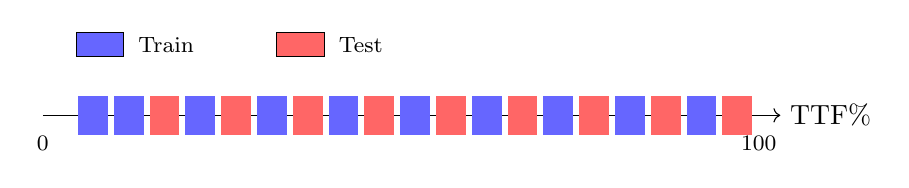
\begin{tikzpicture}[x=0.075\linewidth, y=6mm]
      % Trục TTF
      \draw[->] (0,0) -- (10.3,0) node[right]{TTF\%};
      \node at (0,-0.6){\footnotesize 0}; \node at (10,-0.6){\footnotesize 100};
      
      % Các khối cửa sổ xen kẽ (Train/Test) minh họa rủi ro rò rỉ
      \foreach \x/\c in {0.5/blue!60,1/blue!60,1.5/red!60,2/blue!60,2.5/red!60,3/blue!60,3.5/red!60,4/blue!60,4.5/red!60,5/blue!60,5.5/red!60,6/blue!60,6.5/red!60,7/blue!60,7.5/red!60,8/blue!60,8.5/red!60,9/blue!60,9.5/red!60} {
        \draw[fill=\c,draw=\c] (\x,-0.4) rectangle ++(0.4,0.8);
      }
      
      % Chú thích (Legend) - Phần này làm hình (a) cao hơn hình (b)
      \draw[fill=white, draw=white] (0.5,1.38) rectangle (3.4,1.62);
      \node[draw, fill=blue!60, minimum width=6mm, minimum height=3mm] (l1) at (0.8,1.5) {};
      \node[anchor=west] at (1.2,1.5) {\footnotesize Train};
      \node[draw, fill=red!60, minimum width=6mm, minimum height=3mm] (l2) at (3.6,1.5) {};
      \node[anchor=west] at (4,1.5) {\footnotesize Test};
    \end{tikzpicture}
  \end{minipage}
  \hfill
  \begin{minipage}[b]{0.47\textwidth}
    \centering
    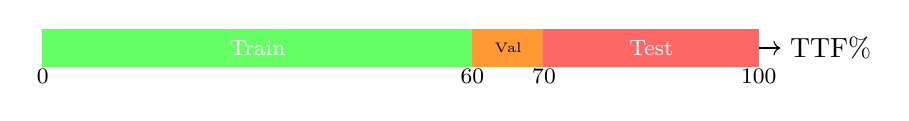
\begin{tikzpicture}[x=0.075\linewidth, y=6mm]
      % Trục TTF
      \draw[->] (0,0) -- (10.3,0) node[right]{TTF\%};
      \node at (0,-0.6){\footnotesize 0}; \node at (6,-0.6){\footnotesize 60}; \node at (7,-0.6){\footnotesize 70}; \node at (10,-0.6){\footnotesize 100};
      
      % Các khối phân chia theo dòng thời gian (Train 60%, Val 10%, Test 30%)
      \draw[fill=green!60,draw=green!60] (0,-0.4) rectangle (6,0.4);
      \node[color=white, font=\footnotesize] at (3,0) {Train};
      
      \draw[fill=orange!80,draw=orange!80] (6,-0.4) rectangle (7,0.4);
      \node[font=\tiny] at (6.5,0) {Val};
      
      \draw[fill=red!60,draw=red!60] (7,-0.4) rectangle (10,0.4);
      \node[color=white, font=\footnotesize] at (8.5,0) {Test};
    \end{tikzpicture}
  \end{minipage}
  
  \caption{Protocol comparison. Left: window-level random split (leakage risk). Right: contiguous TTF\-aligned temporal split (leakage-aware).}
  \label{fig:protocol_compare}
\end{figure}



\section{Results}
\label{sec:results}

\subsection{Stratified evaluation (3-class)}
In the stratified development setting, the best configuration (\texttt{auto\_ft\_r49}) achieves \textbf{Macro-F1 = 0.7762}. 
Per-class F1 scores are approximately: Healthy $\approx$ 0.69, Degrading $\approx$ 0.64, and Fault = 1.00. 
This indicates that Fault signatures are highly separable, while the Degrading stage remains the most challenging due to its transitional nature.

Figure~\ref{fig:strat_pair} summarizes the stratified confusion matrix and per-class F1.

\begin{figure}[t]
  \centering
  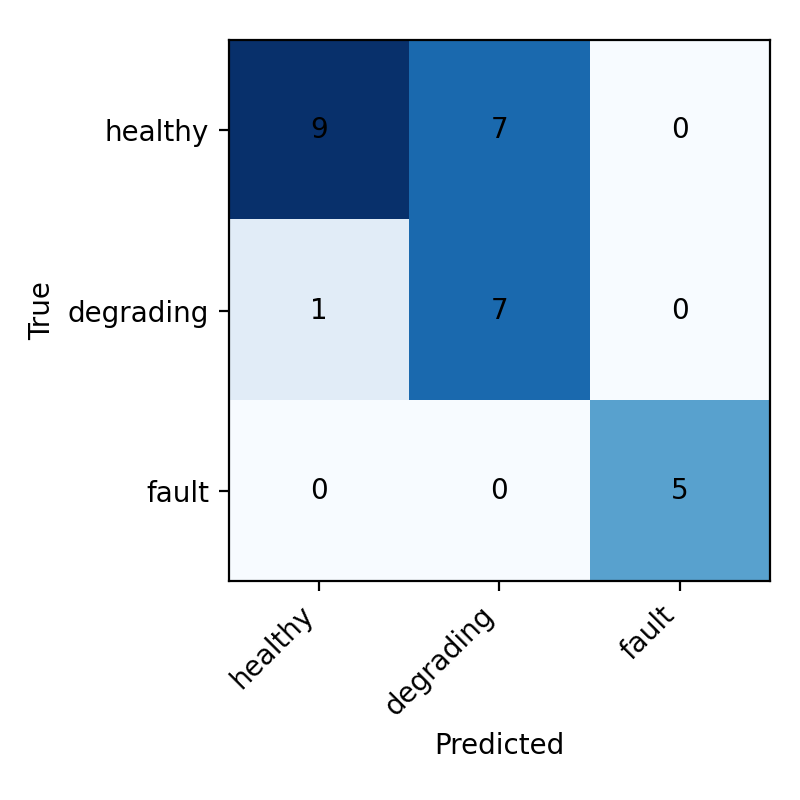
\includegraphics[width=0.48\linewidth]{figures/stratified/confusion_matrix.png}
  \hfill
  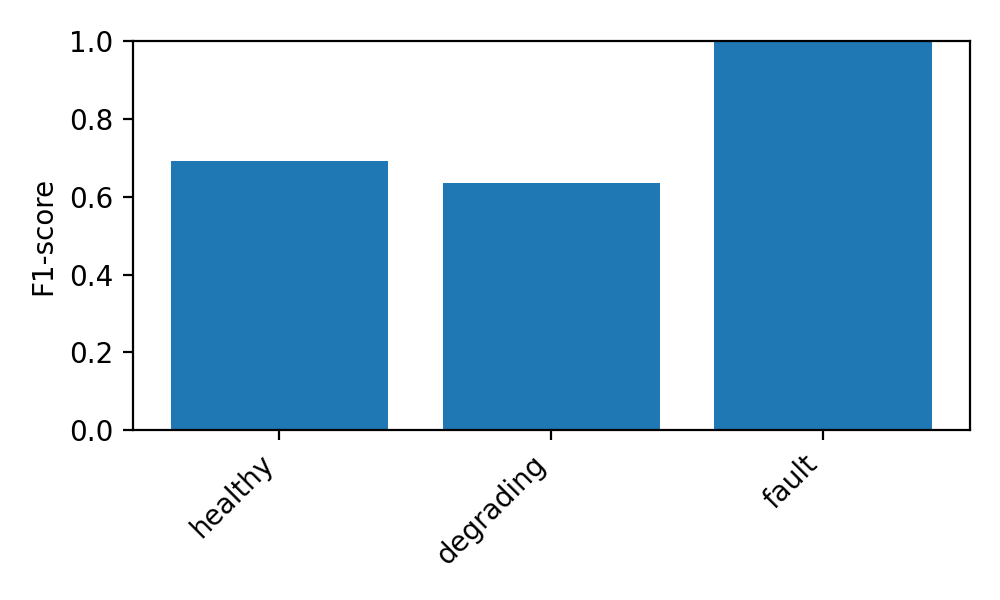
\includegraphics[width=0.48\linewidth]{figures/stratified/f1_per_class.png}
  \caption{Stratified evaluation (3-class). Left: confusion matrix. Right: per-class F1.}
  \label{fig:strat_pair}
\end{figure}

\subsection{Temporal evaluation (deployment-oriented)}
Under the temporal leakage-aware split, the test slice [70,100.1]\% corresponds to late-life behavior where \emph{Healthy samples do not appear}. 
Therefore, metrics are reported over the \emph{present classes} (Degrading and Fault). 
Using mean-logit aggregation, the model attains \textbf{Early (70--90\%): Accuracy = 1.0000 (Degrading only)} and \textbf{Late (90--100\%): Accuracy = 0.3846; Fault F1 = 0.5556}. 
These results suggest that the learned representation transfers from earlier life to late-life conditions, while late Fault recall remains the primary bottleneck.



Figure~\ref{fig:temporal_pair} summarizes temporal performance on the late-life slice.
\begin{figure}[t]
  \centering
  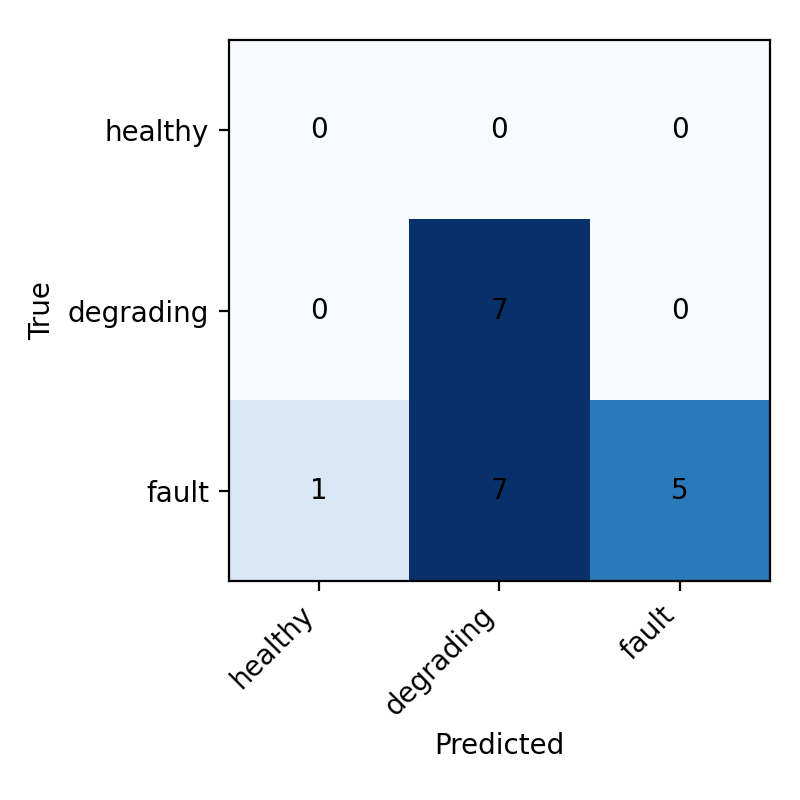
\includegraphics[width=0.48\linewidth]{figures/temporal/confusion_matrix.png}
  \hfill
  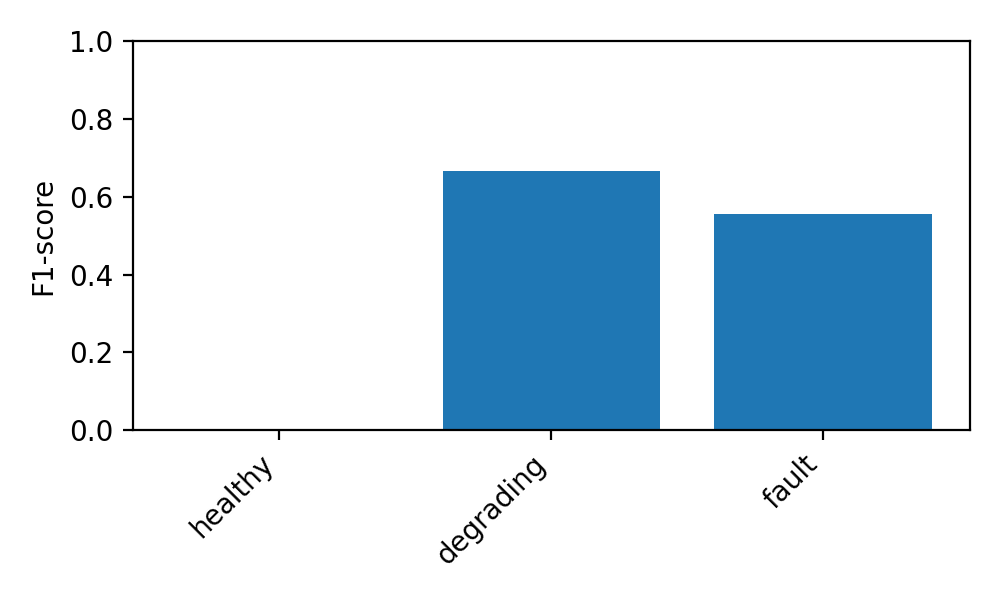
\includegraphics[width=0.48\linewidth]{figures/temporal/f1_per_class.png}
  \caption{Leakage-aware temporal evaluation on the late-life slice [70,100.1]\% TTF (only Degrading and Fault present). Left: confusion matrix. Right: per-class F1 over present classes.}
  \label{fig:temporal_pair}
\end{figure}

\subsection{Full-range temporal (0--100.1\%)}
To assess performance over the entire lifecycle, a full-range temporal evaluation on $[0,100.1]\%$ TTF is conducted. Two file-wise aggregation strategies are compared using the same checkpoint:
\begin{itemize}
  \item Mean aggregation: Accuracy $=0.4806$, Macro-F1 $=0.4907$.
  \item Majority vote: Accuracy $=0.8295$, Macro-F1 $=0.6999$.
\end{itemize}
This comparison highlights a practical trade-off: vote aggregation yields substantially better overall metrics across the full timeline, while mean aggregation retains better late Fault recall on the very-late slice (\S\ref{sec:results}).

\begin{figure}[t]
  \centering
  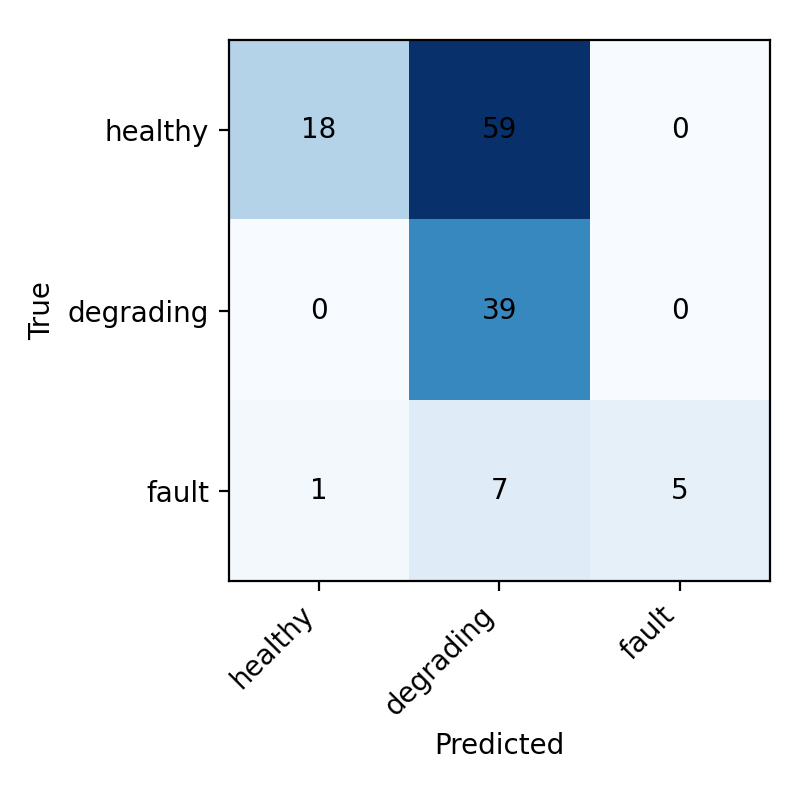
\includegraphics[width=0.48\linewidth]{figures/temporal_alltest/mean_confusion.png}
  \hfill
  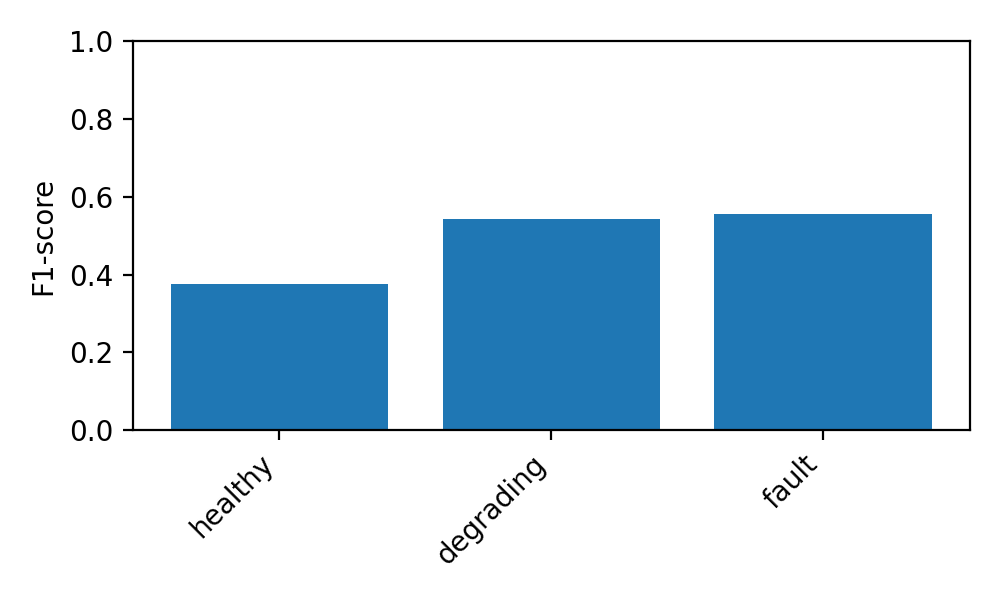
\includegraphics[width=0.48\linewidth]{figures/temporal_alltest/mean_f1.png}
  \caption{Full-range temporal evaluation $[0,100.1]\%$ (mean aggregation). Left: confusion matrix. Right: per-class F1.}
  \label{fig:temporal_alltest_mean}
\end{figure}

\begin{figure}[t]
  \centering
  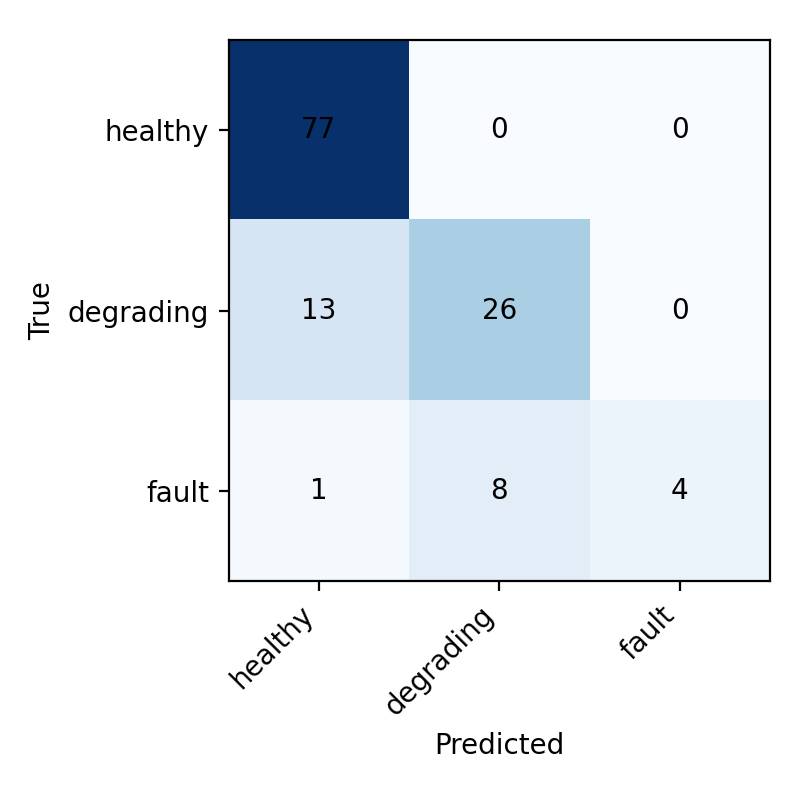
\includegraphics[width=0.48\linewidth]{figures/temporal_alltest/vote_confusion.png}
  \hfill
  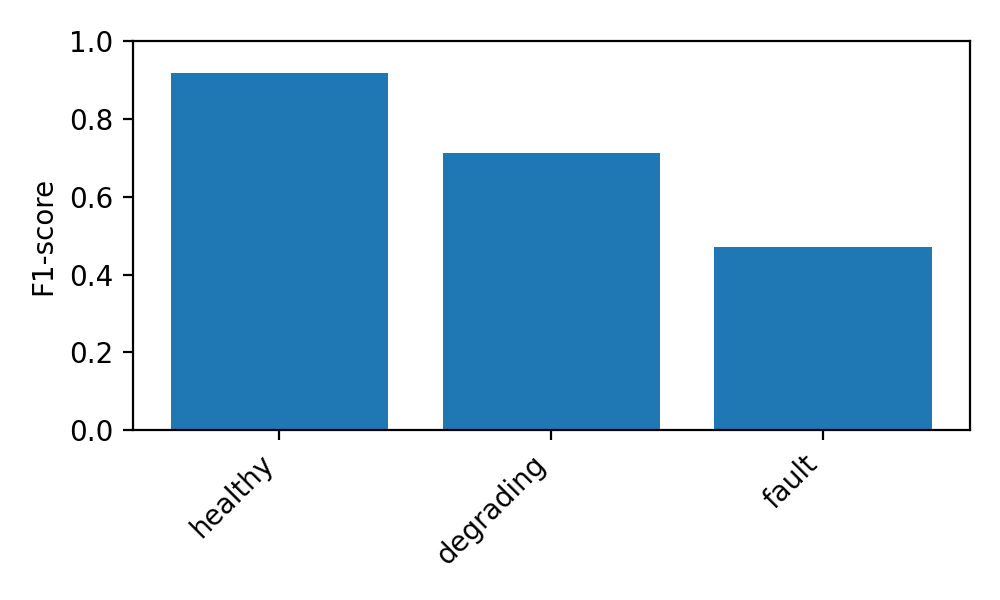
\includegraphics[width=0.48\linewidth]{figures/temporal_alltest/vote_f1.png}
  \caption{Full-range temporal evaluation $[0,100.1]\%$ (majority vote). Left: confusion matrix. Right: per-class F1.}
  \label{fig:temporal_alltest_vote}
\end{figure}

\begin{table}[t]
  \caption{Full-range temporal $[0,100.1]\%$ TTF: mean vs. majority vote aggregation.}
  \label{tab:temporal_alltest_agg}
  \centering
  \begin{tabular}{lcc}
    \toprule
    Aggregation & Accuracy & Macro-F1 \\
    \midrule
    Mean & 0.4806 & 0.4907 \\
    Majority vote & 0.8295 & 0.6999 \\
    \bottomrule
  \end{tabular}
\end{table}

\noindent\textit{Trade-off.} Majority vote substantially improves overall metrics over $[0,100.1]\%$ TTF, while mean-logit aggregation retains better late \textit{Fault} recall on the very-late slice ($[90,100.1]\%$).

\subsection{Failure case analysis with broader temporal coverage}
When expanding evaluation to a broader range that includes more ambiguous mid-life samples, performance drops substantially (Accuracy $\approx$ 0.3333, Macro-F1 $\approx$ 0.3324), where Degrading is frequently confused with Healthy and Healthy may have zero support depending on the slice.  
This behavior highlights that the decision boundary between Healthy and early Degrading is sensitive and requires either (i) stronger supervision/labeling for the transition region, (ii) richer temperature trend modeling, or (iii) sequence-aware modeling that leverages longer temporal context. 

\subsection{Ablation Studies}
\label{sec:ablation}

\paragraph{Effect of stratified initialization.}
Initializing temporal fine-tuning from the best stratified checkpoint yields markedly stronger late-life performance than training from scratch on the same temporal coverage; details omitted for brevity.

\paragraph{Temporal test slice.}
The temporal test slice is further varied to examine protocol effects. A broader late slice $[70,100.1]\%$ includes early Degrading and yields lower Degrading F1 (e.g., 0.07 in this run), while a very-late slice $[90,100.1]\%$ may contain only Fault (macro metrics become less informative). Figure~\ref{fig:abl_slice} shows confusion matrices for both settings.

\noindent (Illustrative confusion plots omitted to save space.)

\paragraph{Multi-modal fusion (vibration + temperature) vs. vibration-only.}
To assess the contribution of temperature features, the multi-modal model is compared against a vibration-only variant where the temperature branch is disabled (same training protocols; stratified pre-training followed by temporal fine-tuning). File-wise metrics on the late-life temporal slice (present-labels) are reported. Table~\ref{tab:mm_vs_vib} summarizes Macro-F1 and Degrading/Fault F1. In the conducted runs, adding the 6-D temperature descriptor improves Degrading recognition while keeping Fault performance high.

\begin{table}[t]
  \caption{Ablation: multi-modal fusion vs. vibration-only on the late-life temporal slice $[85,100.1]\%$ TTF (present-labels). Metrics are computed over present classes (Healthy absent).}
  \label{tab:mm_vs_vib}
  \centering
  \begin{tabular}{lccc}
    \toprule
    Model & Macro-F1 (present) & F1 Degrading & F1 Fault \\
    \midrule
    Vibration-only & 0.2593 & 0.5185 & 0.0000 \\
    Multi-modal (vib+temp) & 0.9467 & 0.9333 & 0.9600 \\
    \bottomrule
  \end{tabular}
\end{table}

\noindent (Confusion plots omitted; see summary table below.)


\paragraph{Broad late slice $[70,100.1]\%$: multi-modal vs. vibration-only.}
To complete the comparison, present-label metrics are also reported on the broader late slice. Here, the vibration-only model emphasizes Degrading (F1 $\approx$ 0.8000) but fails to recognize Fault (F1 $\approx$ 0.0000), while the multi-modal model captures Fault well (F1 $\approx$ 0.9231) but struggles with early Degrading (F1 $\approx$ 0.0741). Table~\ref{tab:mm_vs_vib_broad} summarizes these trends.

\noindent (Broad-slice plots and table omitted; we summarize key late-life metrics below.)

\begin{table}[t]
  \caption{Ablation summary on very-late slice $[90,100.1]\%$ TTF (present-labels).}
  \label{tab:abl_late_summary}
  \centering
  \begin{tabular}{lcc}
    \toprule
    Variant & Accuracy (late) & Fault F1 (late) \\
    \midrule
    Multi-modal (r49, mean) & 0.3846 & 0.5556 \\
    Vib-only & 0.0000 & 0.0000 \\
    No class-weights & 0.3077 & 0.4706 \\
    High-res (4096/1024, 224$\times$224) & 0.8462 & 0.9167 \\
    \bottomrule
  \end{tabular}
\end{table}


\section{Discussion and Threats to Validity}
\label{sec:discussion}

\subsection{Discussion}
The results reinforce two practical observations for run-to-failure bearing monitoring. First, the \textit{Fault} stage is comparatively easier to separate, as late-life vibration signatures often exhibit clear and consistent spectral patterns. In contrast, the \textit{Degrading} stage is intrinsically ambiguous: it represents a transition region where signal changes can be subtle, intermittent, and partially overlapping with Healthy behavior. This is reflected by lower Degrading performance in the stratified 3-class setting and by the confusion observed when evaluation slices include earlier portions of the mid-life region.

Second, the evaluation protocol substantially affects the perceived performance. File-wise stratified splitting is useful for rapid iteration and model selection during development, but it can still overestimate deployment performance when overlapped windows introduce strong temporal correlation. The leakage-aware temporal protocol aligned with the TTF axis provides a more deployment-oriented assessment by enforcing that training data precede validation/testing along the lifetime timeline. Under late-life temporal testing, where only Degrading and Fault are present, the model maintains strong discrimination, suggesting that the learned time--frequency representation transfers from early-life training to later-life conditions when leakage is controlled.

Finally, the multi-modal design provides a simple trade-off between robustness and efficiency. Temperature descriptors add negligible computational overhead relative to the CNN encoder while offering complementary evidence about thermal trends. However, the current 6-D temperature summary is intentionally minimal; richer temporal modeling of temperature (or longer context windows) may further improve sensitivity near the Healthy--Degrading boundary.

\paragraph{What temperature adds.} On the late-life slice $[85,100.1]\%$ TTF, the vibration-only model under-performs (present-label Macro-F1 $\approx$ 0.26) compared with the multi-modal model (Macro-F1 $\approx$ 0.95), primarily due to \emph{Fault} recognition (F1 $\approx$ 0.00 vs. $\approx$ 0.96). This suggests that temperature provides complementary cues about cumulative friction/thermal load that strengthen late-life discrimination when vibration alone is ambiguous or dominated by non-stationary patterns. On the broader late slice $[70,100.1]\%$, a trade-off is observed: vibration-only emphasizes Degrading (F1 $\approx$ 0.80) while multi-modal captures Fault (F1 $\approx$ 0.92), indicating sensor complementarity across sub-regions of the lifecycle.

\subsection{Threats to validity}
\paragraph{Limited run coverage (external validity).}
The experiments are conducted on a single run (RUNS=1) with 129 files, which limits conclusions about generalization across bearings, loads, and operating conditions. A broader evaluation with multiple runs and bearing-wise splits is needed to quantify cross-unit robustness and to assess domain shift.

\paragraph{Stage definitions based on TTF thresholds (construct validity).}
Health stages are defined using fixed TTF thresholds ($\tau_1=0.60$, $\tau_2=0.90$). While practical for structuring a run-to-failure timeline, these thresholds may not perfectly align with the true physical onset of degradation, and the transition region can be inherently fuzzy. Future work could refine labels using additional degradation indicators (e.g., envelope features, kurtosis trends, or expert annotations) and evaluate sensitivity to threshold choices.

\paragraph{Temporal correlation from overlapped windowing (internal validity).}
Window overlap (50\%) increases the number of training instances but also raises the risk of temporal leakage if splits are performed at the window level. This risk is mitigated with a TTF-aligned temporal protocol; nonetheless, residual correlation may remain near split boundaries. Introducing a temporal ``gap'' between train/val/test segments or using non-overlapping evaluation windows are potential safeguards.

\paragraph{Class presence in temporal slices (metric interpretation).}
In late-life temporal testing ([70,100.1]\% TTF), Healthy samples may be absent. Reporting macro metrics over all three classes would be misleading due to zero-support classes. Therefore, performance is reported over the \emph{present classes} for the temporal slice and class coverage is explicitly stated when interpreting results.

\paragraph{Synchronous sampling assumption (deployment validity).}
The current pipeline assumes vibration and temperature are synchronously sampled and windowed using identical indices. If temperature is sampled at a different rate in real deployments, explicit resampling and timestamp alignment will be required before feature extraction. This engineering constraint may affect end-to-end performance and should be validated in future deployments.

\section{Conclusion and Future Work}
\label{sec:conclusion}

This paper investigated three-stage bearing health classification (Healthy, Degrading, Fault) in a run-to-failure setting using a lightweight multi-modal model that fuses STFT-based vibration representations with compact temperature trend descriptors. Beyond a stratified development evaluation, a \textbf{leakage-aware temporal protocol} aligned with the TTF timeline and a two-phase workflow (stratified training $\rightarrow$ temporal fine-tuning) are emphasized to better approximate deployment conditions. Experimental results show strong late-life discrimination between Degrading and Fault under temporal evaluation, while the Healthy--Degrading boundary remains the most challenging region when broader mid-life coverage is included. The choice of TTF thresholds (60\%/90\%) is motivated by empirical observation on this run; the present study is considered a \emph{proof of concept}, and future work will examine threshold sensitivity and validate on additional datasets (e.g., Case Western Reserve University (CWRU), Paderborn) to strengthen generality.

\textbf{Future work} will focus on: (i) extending evaluation to multiple runs/bearings and external datasets (e.g., CWRU, Paderborn), and performing bearing-wise splits to quantify generalization under domain shift; (ii) improving supervision in the transition region via refined degradation indicators or expert-informed labeling beyond fixed TTF thresholds; (iii) incorporating longer temporal context with sequence-aware models to better capture gradual degradation dynamics; and (iv) exploring calibration and uncertainty estimation to support reliable early-warning decisions in practical CBM deployments.

\bmhead{Acknowledgements}
We acknowledge Nguyen Tat Thanh University, Ho Chi Minh City, Vietnam for supporting this study.

\section*{Declarations}

\bmhead{Funding}
Not applicable.

\bmhead{Competing interests}
The authors declare that they have no competing interests.

\bmhead{Ethics approval and consent to participate}
Not applicable.

\bmhead{Consent for publication}
Not applicable.

\bmhead{Data availability}
The dataset used in this study is publicly available \cite{jung2024dib_rtf,jung2024mendeley_rtf}.

\bmhead{Code availability}
Code and configuration files for reproducing the preprocessing, splits, and evaluation will be released upon acceptance.

\bmhead{Author contributions}
Long Truong and Phu Le Nguyen contributed equally to this work. Both authors contributed to conceptualization, methodology, experiments, and writing.

\begingroup
\sloppy
\small
\bibliography{refs}
\endgroup

\end{document}


